\documentclass[]{article}
\usepackage{lmodern}
\usepackage{amssymb,amsmath}
\usepackage{ifxetex,ifluatex}
\usepackage{fixltx2e} % provides \textsubscript
\ifnum 0\ifxetex 1\fi\ifluatex 1\fi=0 % if pdftex
  \usepackage[T1]{fontenc}
  \usepackage[utf8]{inputenc}
\else % if luatex or xelatex
  \ifxetex
    \usepackage{mathspec}
  \else
    \usepackage{fontspec}
  \fi
  \defaultfontfeatures{Ligatures=TeX,Scale=MatchLowercase}
\fi
% use upquote if available, for straight quotes in verbatim environments
\IfFileExists{upquote.sty}{\usepackage{upquote}}{}
% use microtype if available
\IfFileExists{microtype.sty}{%
\usepackage{microtype}
\UseMicrotypeSet[protrusion]{basicmath} % disable protrusion for tt fonts
}{}
\usepackage[margin=1in]{geometry}
\usepackage{hyperref}
\hypersetup{unicode=true,
            pdftitle={Assessment 02 - Quantiles, Percentiles and Boxplots},
            pdfauthor={Alessandro Corradini - Harvard Data Science Professional},
            pdfborder={0 0 0},
            breaklinks=true}
\urlstyle{same}  % don't use monospace font for urls
\usepackage{color}
\usepackage{fancyvrb}
\newcommand{\VerbBar}{|}
\newcommand{\VERB}{\Verb[commandchars=\\\{\}]}
\DefineVerbatimEnvironment{Highlighting}{Verbatim}{commandchars=\\\{\}}
% Add ',fontsize=\small' for more characters per line
\usepackage{framed}
\definecolor{shadecolor}{RGB}{248,248,248}
\newenvironment{Shaded}{\begin{snugshade}}{\end{snugshade}}
\newcommand{\KeywordTok}[1]{\textcolor[rgb]{0.13,0.29,0.53}{\textbf{#1}}}
\newcommand{\DataTypeTok}[1]{\textcolor[rgb]{0.13,0.29,0.53}{#1}}
\newcommand{\DecValTok}[1]{\textcolor[rgb]{0.00,0.00,0.81}{#1}}
\newcommand{\BaseNTok}[1]{\textcolor[rgb]{0.00,0.00,0.81}{#1}}
\newcommand{\FloatTok}[1]{\textcolor[rgb]{0.00,0.00,0.81}{#1}}
\newcommand{\ConstantTok}[1]{\textcolor[rgb]{0.00,0.00,0.00}{#1}}
\newcommand{\CharTok}[1]{\textcolor[rgb]{0.31,0.60,0.02}{#1}}
\newcommand{\SpecialCharTok}[1]{\textcolor[rgb]{0.00,0.00,0.00}{#1}}
\newcommand{\StringTok}[1]{\textcolor[rgb]{0.31,0.60,0.02}{#1}}
\newcommand{\VerbatimStringTok}[1]{\textcolor[rgb]{0.31,0.60,0.02}{#1}}
\newcommand{\SpecialStringTok}[1]{\textcolor[rgb]{0.31,0.60,0.02}{#1}}
\newcommand{\ImportTok}[1]{#1}
\newcommand{\CommentTok}[1]{\textcolor[rgb]{0.56,0.35,0.01}{\textit{#1}}}
\newcommand{\DocumentationTok}[1]{\textcolor[rgb]{0.56,0.35,0.01}{\textbf{\textit{#1}}}}
\newcommand{\AnnotationTok}[1]{\textcolor[rgb]{0.56,0.35,0.01}{\textbf{\textit{#1}}}}
\newcommand{\CommentVarTok}[1]{\textcolor[rgb]{0.56,0.35,0.01}{\textbf{\textit{#1}}}}
\newcommand{\OtherTok}[1]{\textcolor[rgb]{0.56,0.35,0.01}{#1}}
\newcommand{\FunctionTok}[1]{\textcolor[rgb]{0.00,0.00,0.00}{#1}}
\newcommand{\VariableTok}[1]{\textcolor[rgb]{0.00,0.00,0.00}{#1}}
\newcommand{\ControlFlowTok}[1]{\textcolor[rgb]{0.13,0.29,0.53}{\textbf{#1}}}
\newcommand{\OperatorTok}[1]{\textcolor[rgb]{0.81,0.36,0.00}{\textbf{#1}}}
\newcommand{\BuiltInTok}[1]{#1}
\newcommand{\ExtensionTok}[1]{#1}
\newcommand{\PreprocessorTok}[1]{\textcolor[rgb]{0.56,0.35,0.01}{\textit{#1}}}
\newcommand{\AttributeTok}[1]{\textcolor[rgb]{0.77,0.63,0.00}{#1}}
\newcommand{\RegionMarkerTok}[1]{#1}
\newcommand{\InformationTok}[1]{\textcolor[rgb]{0.56,0.35,0.01}{\textbf{\textit{#1}}}}
\newcommand{\WarningTok}[1]{\textcolor[rgb]{0.56,0.35,0.01}{\textbf{\textit{#1}}}}
\newcommand{\AlertTok}[1]{\textcolor[rgb]{0.94,0.16,0.16}{#1}}
\newcommand{\ErrorTok}[1]{\textcolor[rgb]{0.64,0.00,0.00}{\textbf{#1}}}
\newcommand{\NormalTok}[1]{#1}
\usepackage{graphicx,grffile}
\makeatletter
\def\maxwidth{\ifdim\Gin@nat@width>\linewidth\linewidth\else\Gin@nat@width\fi}
\def\maxheight{\ifdim\Gin@nat@height>\textheight\textheight\else\Gin@nat@height\fi}
\makeatother
% Scale images if necessary, so that they will not overflow the page
% margins by default, and it is still possible to overwrite the defaults
% using explicit options in \includegraphics[width, height, ...]{}
\setkeys{Gin}{width=\maxwidth,height=\maxheight,keepaspectratio}
\IfFileExists{parskip.sty}{%
\usepackage{parskip}
}{% else
\setlength{\parindent}{0pt}
\setlength{\parskip}{6pt plus 2pt minus 1pt}
}
\setlength{\emergencystretch}{3em}  % prevent overfull lines
\providecommand{\tightlist}{%
  \setlength{\itemsep}{0pt}\setlength{\parskip}{0pt}}
\setcounter{secnumdepth}{0}
% Redefines (sub)paragraphs to behave more like sections
\ifx\paragraph\undefined\else
\let\oldparagraph\paragraph
\renewcommand{\paragraph}[1]{\oldparagraph{#1}\mbox{}}
\fi
\ifx\subparagraph\undefined\else
\let\oldsubparagraph\subparagraph
\renewcommand{\subparagraph}[1]{\oldsubparagraph{#1}\mbox{}}
\fi

%%% Use protect on footnotes to avoid problems with footnotes in titles
\let\rmarkdownfootnote\footnote%
\def\footnote{\protect\rmarkdownfootnote}

%%% Change title format to be more compact
\usepackage{titling}

% Create subtitle command for use in maketitle
\newcommand{\subtitle}[1]{
  \posttitle{
    \begin{center}\large#1\end{center}
    }
}

\setlength{\droptitle}{-2em}

  \title{Assessment 02 - Quantiles, Percentiles and Boxplots}
    \pretitle{\vspace{\droptitle}\centering\huge}
  \posttitle{\par}
    \author{Alessandro Corradini - Harvard Data Science Professional}
    \preauthor{\centering\large\emph}
  \postauthor{\par}
    \date{}
    \predate{}\postdate{}
  

\begin{document}
\maketitle

\subsection{\texorpdfstring{\textbf{Vector
lengths}}{Vector lengths}}\label{vector-lengths}

When analyzing data it's often important to know the number of
measurements you have for each category.

\textbf{Instructions}

\begin{itemize}
\tightlist
\item
  Define a variable \texttt{male} that contains the male heights.
\item
  Define a variable \texttt{female} that contains the female heights.
\item
  Report the length of each variable.
\end{itemize}

\begin{Shaded}
\begin{Highlighting}[]
\KeywordTok{library}\NormalTok{(dslabs)}
\KeywordTok{data}\NormalTok{(heights)}
\NormalTok{male <-}\StringTok{ }\NormalTok{heights}\OperatorTok{$}\NormalTok{height[heights}\OperatorTok{$}\NormalTok{sex}\OperatorTok{==}\StringTok{"Male"}\NormalTok{]}
\NormalTok{female <-}\StringTok{ }\NormalTok{heights}\OperatorTok{$}\NormalTok{height[heights}\OperatorTok{$}\NormalTok{sex}\OperatorTok{==}\StringTok{"Female"}\NormalTok{]}
\KeywordTok{length}\NormalTok{(male)}
\end{Highlighting}
\end{Shaded}

\begin{verbatim}
## [1] 812
\end{verbatim}

\begin{Shaded}
\begin{Highlighting}[]
\KeywordTok{length}\NormalTok{(female)}
\end{Highlighting}
\end{Shaded}

\begin{verbatim}
## [1] 238
\end{verbatim}

\subsection{\texorpdfstring{\textbf{Percentiles}}{Percentiles}}\label{percentiles}

Suppose we can't make a plot and want to compare the distributions side
by side. If the number of data points is large, listing all the numbers
is inpractical. A more practical approach is to look at the percentiles.
We can obtain percentiles using the \texttt{quantile} function like this

\begin{verbatim}
library(dslabs)
data(heights)
quantile(heights$height, seq(.01, 0.99, 0.01))
\end{verbatim}

\textbf{Instructions}

\begin{itemize}
\tightlist
\item
  Create two five row vectors showing the 10th, 30th, 50th, 70th, and
  90th percentiles for the heights of each sex called these vectors
  \texttt{female\_percentiles} and \texttt{male\_percentiles}.
\item
  Then create a data frame called \texttt{df} with these two vectors as
  columns. The column names should be \texttt{female} and \texttt{male}
  and should appear in that order. As an example consider that if you
  want a data frame to have column names \texttt{names} and
  \texttt{grades}, in that order, you do it like this:
\end{itemize}

\begin{verbatim}
df <- data.frame(names = c("Jose", "Mary"), grades = c("B", "A"))
\end{verbatim}

\begin{itemize}
\tightlist
\item
  Take a look at the \texttt{df} by printing it. This will provide some
  information on how male and female heights differ.
\end{itemize}

\begin{Shaded}
\begin{Highlighting}[]
\KeywordTok{library}\NormalTok{(dslabs)}
\KeywordTok{data}\NormalTok{(heights)}
\NormalTok{male <-}\StringTok{ }\NormalTok{heights}\OperatorTok{$}\NormalTok{height[heights}\OperatorTok{$}\NormalTok{sex}\OperatorTok{==}\StringTok{"Male"}\NormalTok{]}
\NormalTok{female <-}\StringTok{ }\NormalTok{heights}\OperatorTok{$}\NormalTok{height[heights}\OperatorTok{$}\NormalTok{sex}\OperatorTok{==}\StringTok{"Female"}\NormalTok{]}

\NormalTok{male_percentiles <-}\StringTok{ }\KeywordTok{quantile}\NormalTok{(male, }\KeywordTok{c}\NormalTok{(.}\DecValTok{1}\NormalTok{,.}\DecValTok{3}\NormalTok{,.}\DecValTok{5}\NormalTok{,.}\DecValTok{7}\NormalTok{,.}\DecValTok{9}\NormalTok{))}
\NormalTok{female_percentiles <-}\StringTok{ }\KeywordTok{quantile}\NormalTok{(female, }\KeywordTok{c}\NormalTok{(.}\DecValTok{1}\NormalTok{,.}\DecValTok{3}\NormalTok{,.}\DecValTok{5}\NormalTok{,.}\DecValTok{7}\NormalTok{,.}\DecValTok{9}\NormalTok{))}

\NormalTok{df <-}\StringTok{ }\KeywordTok{data.frame}\NormalTok{(}\DataTypeTok{female =}\NormalTok{ female_percentiles, }\DataTypeTok{male =}\NormalTok{ male_percentiles)}

\KeywordTok{print}\NormalTok{(df)}
\end{Highlighting}
\end{Shaded}

\begin{verbatim}
##       female     male
## 10% 61.00000 65.00000
## 30% 63.00000 68.00000
## 50% 64.98031 69.00000
## 70% 66.46417 71.00000
## 90% 69.00000 73.22751
\end{verbatim}

\subsection{\texorpdfstring{\textbf{Interpretating Boxplots -
1}}{Interpretating Boxplots - 1}}\label{interpretating-boxplots---1}

Study the boxplots summarizing the distributions of populations sizes by
country.

\begin{figure}
\centering
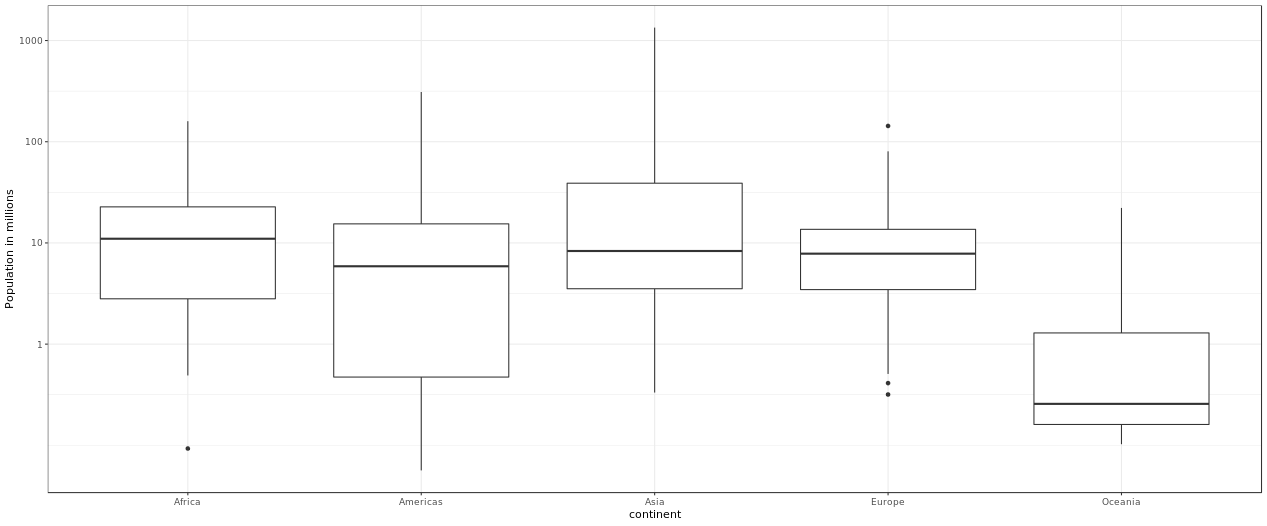
\includegraphics{img1.png}
\caption{}
\end{figure}

Which continent has the country with the largest population size?

\textbf{Instructions}

Possible Answers

\begin{itemize}
\tightlist
\item
  Africa
\item
  Americas
\item
  Asia {[}X{]}
\item
  Europe
\item
  Oceania
\end{itemize}

\subsection{\texorpdfstring{\textbf{NInterpretating Boxplots -
2}}{NInterpretating Boxplots - 2}}\label{ninterpretating-boxplots---2}

Study the boxplots summarizing the distributions of populations sizes by
country.

\begin{figure}
\centering
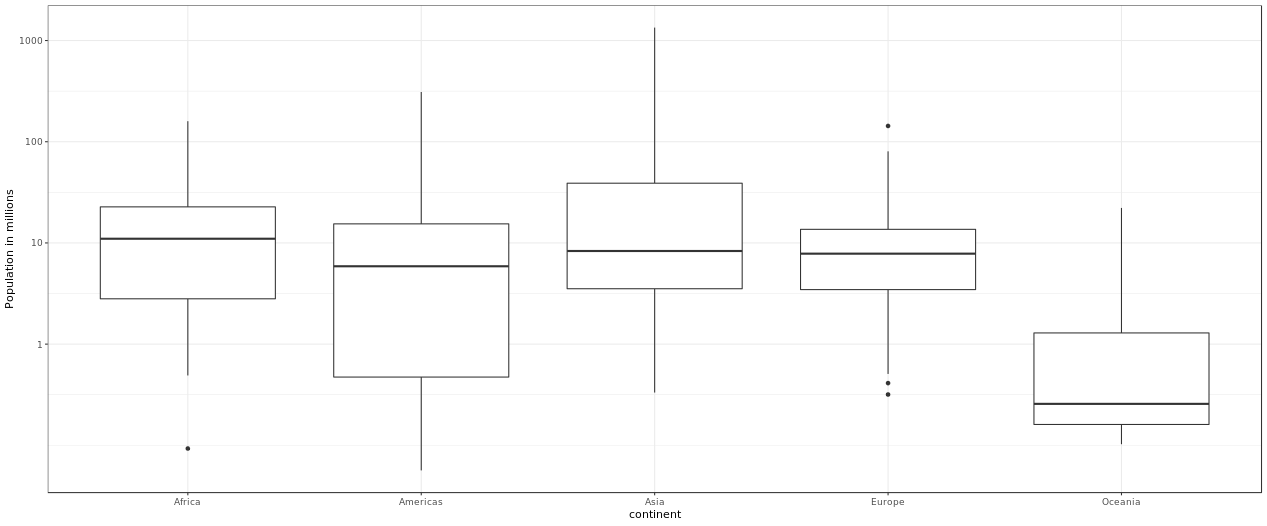
\includegraphics{img1.png}
\caption{}
\end{figure}

Which continent has median country with the largest population?

\textbf{Instructions}

Possible Answers

\begin{itemize}
\tightlist
\item
  Africa {[}X{]}
\item
  Americas
\item
  Asia
\item
  Europe
\item
  Oceania
\end{itemize}

\subsection{\texorpdfstring{\textbf{Interpreting Boxplots -
3}}{Interpreting Boxplots - 3}}\label{interpreting-boxplots---3}

Again, look at the boxplots summarizing the distributions of populations
sizes by country. To the nearest million, what is the \texttt{median}
population size for Africa?

\begin{figure}
\centering
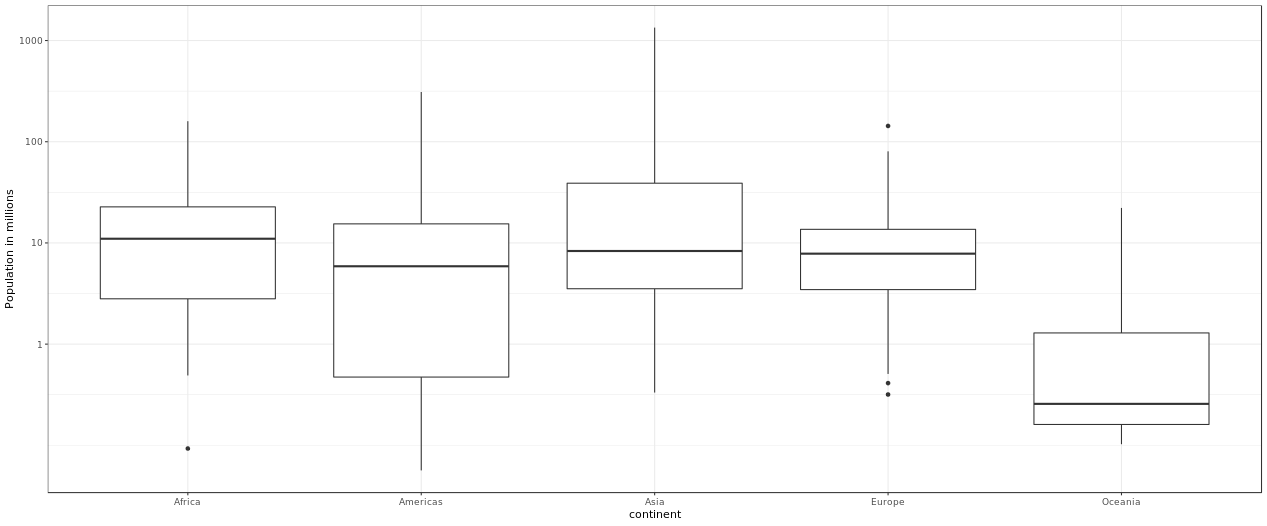
\includegraphics{img1.png}
\caption{}
\end{figure}

\textbf{Instructions}

Possible Answers

\begin{itemize}
\tightlist
\item
  100 million
\item
  25 million
\item
  10 million {[}X{]}
\item
  5 million
\item
  1 million
\end{itemize}

\subsection{\texorpdfstring{\textbf{Low
quantiles}}{Low quantiles}}\label{low-quantiles}

Examine the following boxplots and report approximately what proportion
of countries in Europe have populations below 14 million:

\begin{figure}
\centering
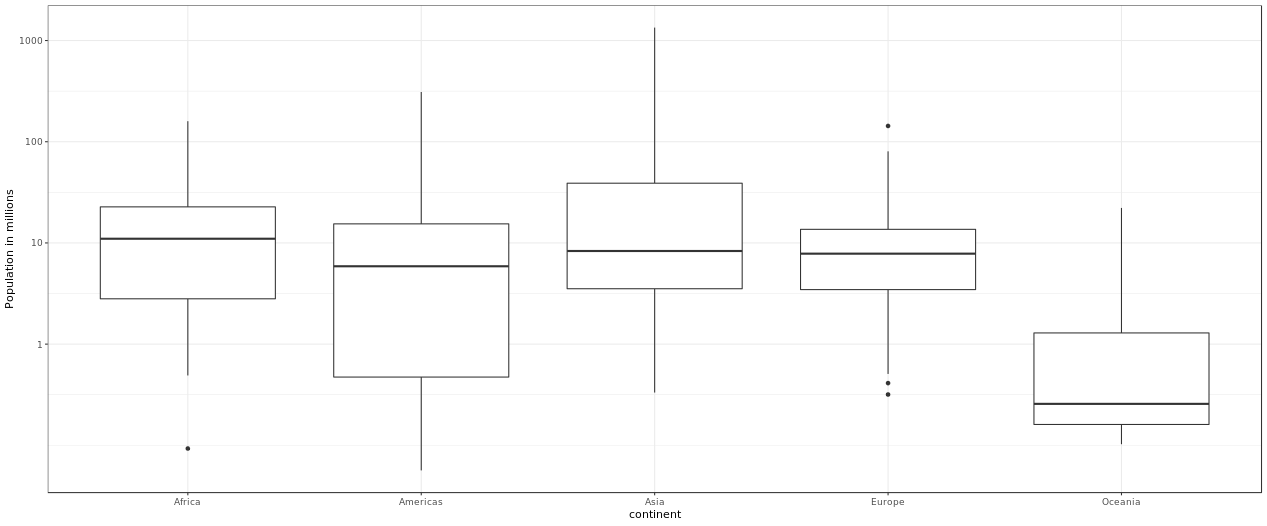
\includegraphics{img1.png}
\caption{}
\end{figure}

Instructions

Possible Answers

\begin{itemize}
\tightlist
\item
  0.75 {[}X{]}
\item
  0.50
\item
  0.25
\item
  0.01
\end{itemize}

\subsection{\texorpdfstring{\textbf{Interquantile Range
(IQR)}}{Interquantile Range (IQR)}}\label{interquantile-range-iqr}

Based on the boxplot, if we use a log transformation, which continent
shown below has the largest interquartile range?

\begin{figure}
\centering
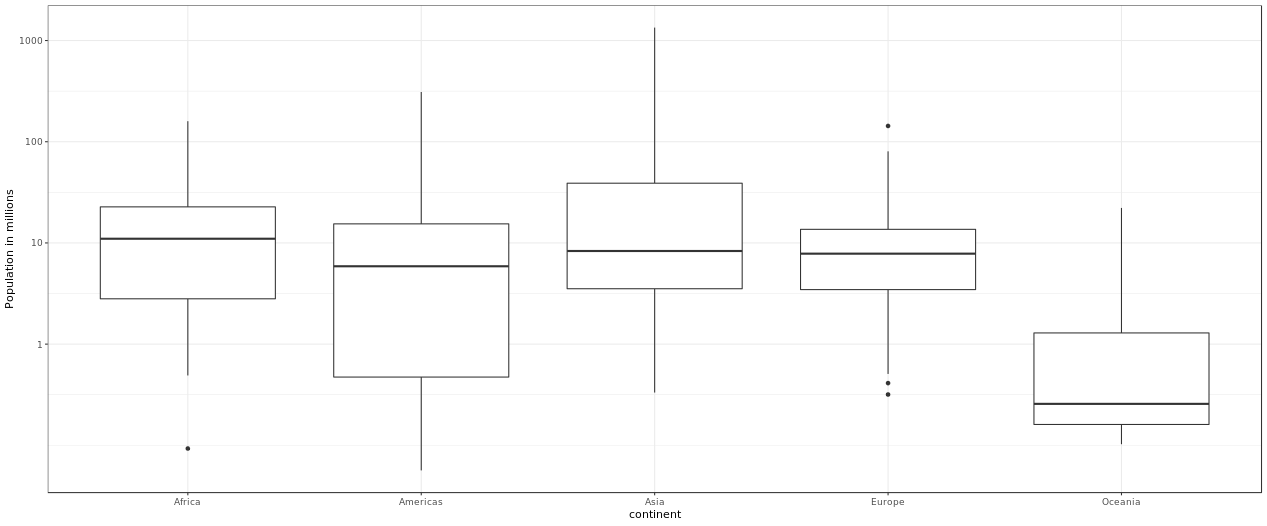
\includegraphics{img1.png}
\caption{}
\end{figure}

\textbf{Instructions}

Possible Answers

\begin{itemize}
\tightlist
\item
  Africa
\item
  Americas {[}X{]}
\item
  Asia
\item
  Europe
\item
  Oceania
\end{itemize}


\end{document}
